\documentclass[border=8pt]{standalone}
% shared preamble for lecture topic figures (compile from beamer/ with xelatex)
\usepackage{tikz}
\usepackage{fontspec}
\usepackage{amsmath}
\usetikzlibrary{arrows.meta,positioning,calc,backgrounds,fit,decorations.pathmorphing}
\setsansfont{SpaceGrotesk}[Path=fonts/,Extension=.ttf,UprightFont=*-400,BoldFont=*-700,FontFace={md}{n}{*-500}]
\renewcommand{\familydefault}{\sfdefault}
\definecolor{navy}{HTML}{182B49}
\definecolor{gold}{HTML}{C8881E}
\definecolor{teal}{HTML}{1F6F86}
\definecolor{green}{HTML}{157E6B}
\definecolor{stone}{HTML}{F7F6F2}
\definecolor{ink}{HTML}{182B49}
\tikzset{
  card/.style={fill=white, rounded corners=4pt, draw=navy!15, line width=0.5pt},
  flow/.style={-{Stealth[length=4pt]}, navy, line width=0.9pt},
  lab/.style={text=navy, font=\sffamily\fontsize{8}{9}\selectfont},
  toplab/.style={text=navy!65, font=\sffamily\fontsize{8.5}{10}\selectfont},
}

\begin{document}
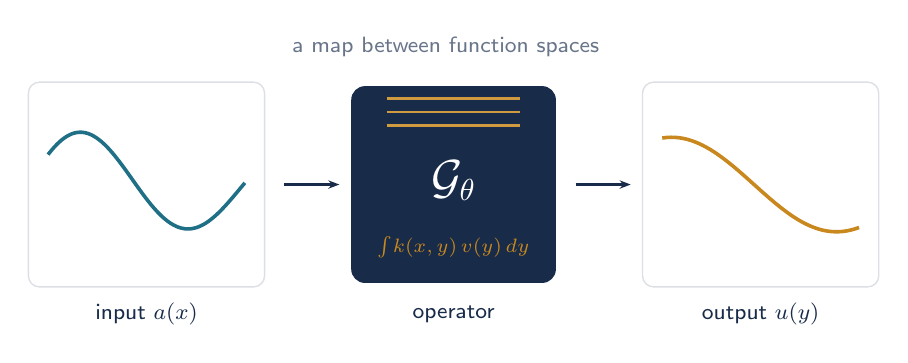
\begin{tikzpicture}
  \node[toplab] at (5.3,3.05) {a map between function spaces};
  % input function card
  \path[card] (0,0) rectangle (3,2.6);
  \draw[teal, line width=1.3pt] plot[domain=0.25:2.75,samples=70]
    (\x,{1.3+0.72*sin(deg(2.3*\x))*exp(-0.12*\x)});
  \node[lab] at (1.5,-0.35) {input $a(x)$};

  \draw[flow] (3.25,1.3) -- (3.95,1.3);

  % operator block
  \begin{scope}[shift={(4.1,0)}]
    \fill[navy, rounded corners=5pt] (0,0.05) rectangle (2.6,2.55);
    \foreach \i in {0,1,2}{\draw[gold!85, line width=0.9pt] (0.45,{2.05+\i*0.17}) -- (2.15,{2.05+\i*0.17});}
    \node[white, font=\sffamily\bfseries\fontsize{16}{17}\selectfont] at (1.3,1.35) {$\mathcal{G}_\theta$};
    \node[gold, font=\sffamily\fontsize{7}{8}\selectfont] at (1.3,0.5) {$\int\! k(x,y)\,v(y)\,dy$};
    \node[lab, text=navy] at (1.3,-0.35) {operator};
  \end{scope}

  \draw[flow] (6.95,1.3) -- (7.65,1.3);

  % output function card
  \begin{scope}[shift={(7.8,0)}]
    \path[card] (0,0) rectangle (3,2.6);
    \draw[gold, line width=1.3pt] plot[domain=0.25:2.75,samples=70]
      (\x,{1.3+0.6*sin(deg(1.5*\x+45))});
    \node[lab] at (1.5,-0.35) {output $u(y)$};
  \end{scope}
\end{tikzpicture}
\end{document}
